% Created 2023-09-30 sáb 18:07
% Intended LaTeX compiler: pdflatex
\documentclass[11pt]{article}
\usepackage[utf8]{inputenc}
\usepackage[T1]{fontenc}
\usepackage{graphicx}
\usepackage{grffile}
\usepackage{longtable}
\usepackage{wrapfig}
\usepackage{rotating}
\usepackage[normalem]{ulem}
\usepackage{amsmath}
\usepackage{textcomp}
\usepackage{amssymb}
\usepackage{capt-of}
\usepackage{hyperref}
\usepackage{../modern}
\bibliography{./sources.bib}
\raggedbottom
\setcounter{secnumdepth}{2}
\author{Luis Eduardo Galindo Amaya (1274895)}
\date{25 de Septiembre 2023}
\title{¿Como fortalecer un servidor Linux y Windows?}
\hypersetup{
 pdfauthor={Luis Eduardo Galindo Amaya (1274895)},
 pdftitle={¿Como fortalecer un servidor Linux y Windows?},
 pdfkeywords={},
 pdfsubject={},
 pdfcreator={Emacs 27.1 (Org mode 9.3)}, 
 pdflang={Spanish}}
\begin{document}

\modentitlepage{../images/escudo-uabc-2022-1-tinta-pos.png}
\tableofcontents
\pagebreak
\datasection{Individual}

\section{Lista de verificación de refuerzo Linux}
\label{sec:org76e30e7}
\cite{lista_linux}

\begin{enumerate}
\item Deshabilitar SSH
\item Deshabilitar acceso raíz SSH
\item Cambiar puerto predeterminado de SSH
\item Deshabilitar la autenticación de contraseña SSH
\item Definir las reglas adecuadas de Nftables o Iptables
\item Implementar IDS (Sistema de detección de intrusos)
\item Asegurar el BIOS
\item Cifrar dispositivos de almacenamiento y particiones
\item Proteja el sistema contra rootkits
\item Mantenga el sistema actualizado
\item VPN (red privada virtual)
\item Habilitar SELinux (Linux con seguridad mejorada)
\item Implementar Honeypots y Honeynets
\item Análisis externo de su dispositivo en busca de vulnerabilidades
\end{enumerate}

\section{Lista de verificación de refuerzo Windows}
\label{sec:orgeea3405}
\cite{Alex_2021}

\begin{enumerate}
\item Nunca conecte un servidor IIS a Internet hasta que esté completamente protegido.
\item Coloque el servidor en un lugar físicamente seguro.
\item Utilice dos interfaces de red en el servidor: una para el administrador y otra para la red.
\item Instale service packs, parches y hotfix.
\item Ejecute el kit de herramientas de cumplimiento de seguridad de Microsoft.
\item Ejecute IIS Lockdown en el servidor
\item Deshabilite los servicios de Windows innecesarios.
\item Asegúrese de que los servicios se ejecuten con los privilegios mínimos cuentas.
\item Desactive el servicio Telnet.
\item Desactive el servicio de estado ASP.NET si no lo utilizan sus aplicaciones.
\item Desactive la creación y el control de versiones distribuidos en la web si la aplicación no lo utiliza, o asegúrelo si es necesario.
\item No instale Microsoft Data Access Components (MDAC) a menos que sea específicamente necesario.
\item No instale la versión HTML de Internet Services Manager.
\item No instale Microsoft Index Server a menos que sea necesario.
\item No instale Microsoft FrontPage Server Extensions (FPSE) a menos que sea necesario.
\item Fortalezca la pila de TCP / IP.
\item Desactive NetBIOS y el bloque de mensajes del servidor: cierre los puertos 137, 138, 139 y 445.
\item Reconfigure las políticas de datos del sistema de archivos de páginas y papelera de reciclaje.
\item Configuración segura de CMOS (semiconductor complementario de óxido de metal).
\item Medios físicos seguros: unidad de CD-ROM, etc.
\end{enumerate}

\section{Diagrma}
\label{sec:org1afe990}
\begin{center}
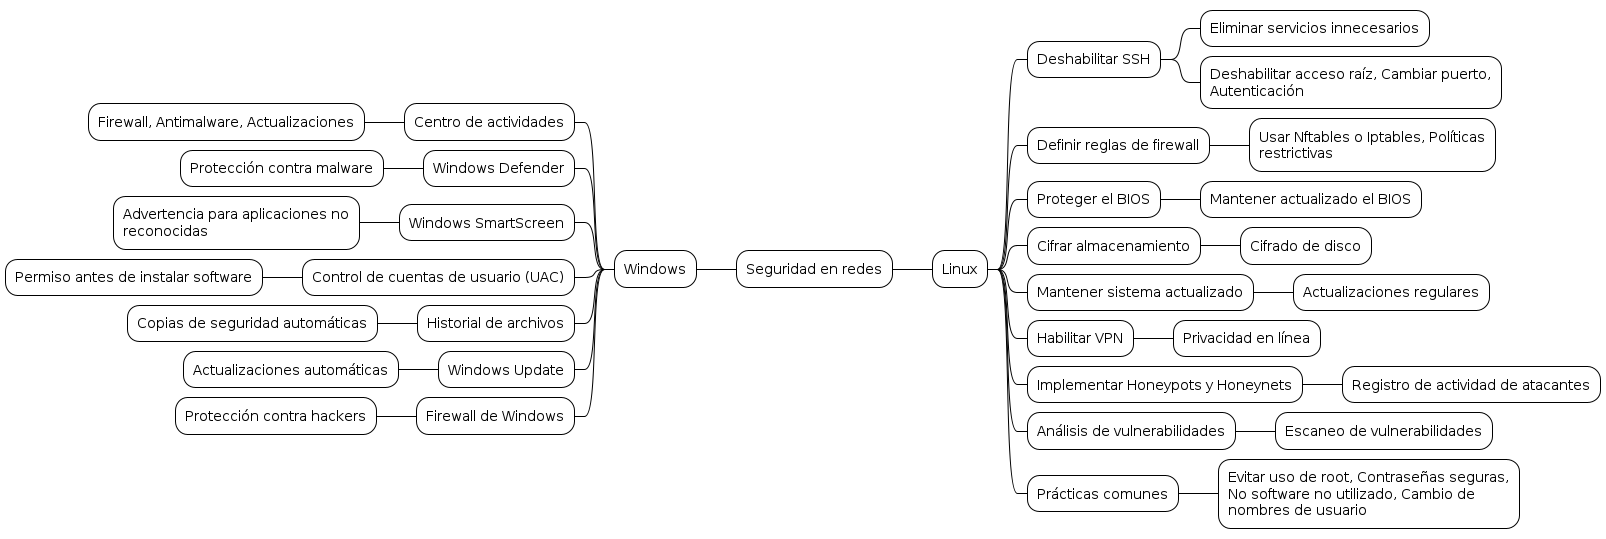
\includegraphics[width=.9\linewidth]{a.png}
\end{center}

\section{Conclusión}
\label{sec:orgb036a76}
A lo largo de esta practica aprendi que cosas se deben tomar en cuenta para mantener un sistema
operativo de manera segura, con la simplicidad de intara un sistema operativo hoy en dia se puede
dar espacio no configurar adecuadamente los acesso al sistema.

\section{Referencias}
\label{sec:org69b6b90}
\printbibliography[heading=none]
\end{document}
